


\chapter{Background} \label{chap:background}

This chapter introduces the tools and techniques used in this thesis. We will briefly describe all the feature of DSP-C in first section. Second section concentrates on contract based programming. Third section explains satisfiability (SAT) techniques. Fourth section describes features and architectures of CBMC.


\section{DSP-C}\index{DSP-C}\label{sec:back:dspc}

As the name suggests DSP-C is a programming language extension proposed by a private company, Associated Compiler Experts (ACE). It is an extension to ISO/IEC IS 9899:1900 (ISO C) standard to support the hardware features of Digital Signal Processors (DSP's) \cite{website:dspc:specification}. These extensions are proposed to overcome the standard C language's inability to handle divided memory spaces, circular buffers, dedicated register sets, fixed point data-types and fixed point arithmetic \cite{dspcbenifits}.

\subsection{Fixed point}

Computing machines like calculators, computers or embedded controllers represent all the numbers in binary. Integers can be directly mapped to finite bit stream of binary digits. Common way to represent fractions is using \emph{floating points} or \emph{fixed point}. Floating point arithmetic supports wider range of values as it has "floating" decimal point. The number is represented using \emph{significant} and \emph{exponent}. \cite{overton2001numerical} presents the various advantages and disadvantage of floating point numbers. Commonly embedded systems do not support floating point values since floating point arithmetic require large logic, needs more computation time and energy \cite{tiwari1995power}. Common alternative is to use fixed point values. Fixed point use fixed number of digits after decimal point. Fixed point values are stored similar to integer values and the decimal position is known since its constant.

\subsection{Fixed point data type}

Programmers can use fixed point data types as easily as any other data types in C language, to describe fixed point arithmetic operations. Explicit support for fixed point types in programming language will allow compiler developers to design fixed point specific optimisations in compilers \cite{dspcbenifits}. It also provides a standardised mechanism to define and use fixed point data types.

DSP-C defines the following fixed point data types:

\subsubsection{̣\_\_fixed types}\index{\_\_fixed}\index{\_\_fixed}
Signed \_\_fixed and unsigned \_\_fixed types will have a mantissa value. A \_\_fixed object represents values in the range of [-1.0, +1.0]. Number of bits used to store a \_\_fixed is platform specific. For example, a platform specific variant of \_\_fixed type is defined in \autoref{tab:fixedtypeexample}. Similarly, a platform may define short \_\_fixed to be 16 bits.

\begin{table}[htbp]
\centering
    \begin{tabular}{ | l | p{0.75cm} | l | p{2cm} |}
    \hline
    \textbf{Type}  & \textbf{Size in bits} & \textbf{Value range} & \textbf{Step size (least value greater than 0)} \\ \hline
    short \_\_fixed           & 8    & -1.0r to 0.9921875r  & 0.0078125r \\ \hline
    unsigned short \_\_fixed  & 7    & 0.0ur to 0.9921875r & 0.0078215ur\\ \hline
    \_\_fixed                 & 16   & -1.0r to 0.99996928..r & 0.000030..r\\ \hline
    unsigned \_\_fixed        & 15   & 0.0r to 0.99996928..ur & 0.000030..ur\\ \hline

    \end{tabular}
\caption{A platform specific definition of \_\_fixed types}
[NOTE: Succeeding `r' and `ur' in above value ranges represents a \_\_fixed type signed and unsigned constants, respectively.]
\label{tab:fixedtypeexample}
\end{table}

\subsubsection{̣\_\_accum types}\index{\_\_accum}
The \_\_accum type is similar to \_\_fixed type with extra 8bits bits to store value before decimal point. For example \_\_accum can store 3.142, but \_\_fixed can only store values between [-1, +1], like 0.142. DSP-C specification \cite{website:dspc:specification} defines that ``\_\_accum type shall have the same scaling factors as the corresponding \_\_fixed types, with an extension of 8 bits, an \_\_accum value can represent value between [-256.0 to +256.0]". For example, a platform specific variant of \_\_accum type is defined in \autoref{tab:accumtypeexample}.

\begin{table}[htbp]
\centering
    \begin{tabular}{ | l | p{0.75cm} | l | p{2cm} |}
    \hline
    \textbf{Type}  & \textbf{Size in bits} & \textbf{Value range} & \textbf{Step size (least value greater than 0)} \\ \hline
    short \_\_accum           & 16    & -256.0a to 255.9921875a  & 0.0078125a \\ \hline
    unsigned short \_\_fixed  & 15    & 0.0ua to 511.9921875ua & 0.0078215ua\\ \hline
    \_\_fixed                 & 24   & -256.0a to 255.99996928..a & 0.000030..a\\ \hline
    unsigned \_\_fixed        & 23   & 0.0r to 511.99996928..ua & 0.000030..ua\\ \hline

    \end{tabular}
\caption{A platform specific definition of \_\_accum types}
[NOTE: Succeeding `a' and `ua' in above value ranges represents a \_\_accum type signed and unsigned constants, respectively.]
\label{tab:accumtypeexample}
\end{table}

\subsubsection{Operations on new data types} \index{\_\_sat}
DSP-C also defines operations and behaviours of all the operations on data types. It supports all standard C operations on new data types, such as arithmetic operations, logical operations, relational operations and a special qualifier. A special qualifier is \_\_sat, which is only applicable to the \_\_fixed type, makes a \_\_fixed into \_\_sat a qualified value, which is used during the expression evaluation phase \cite{website:dspc:specification}. The sat qualifier adds a saturation operation to expressions. The saturation operation returns same value if the value is less than maximum storable value in  \_\_fixed type, otherwise it returns maximum storable value. This operation avoids over flow conditions.

\subsection{Divided memory spaces} \label{sec:memory:lable}

DSP-C allows programmers to provide distributed memory views to compilers. Since memories in DSP's can be physically located in different places, providing divided memory view to developer gives them flexibility to decide on memory location for each variable. This is achieved through memory labelling. When a variable is defined, the label on definition tells compiler which memory will hold a particular variable.

\textbf{Example}
\begin{lstlisting}
__X  int a;
__Y  int b;
\end{lstlisting}

In above example, variable $a$ and $b$ may be allocated in different memory regions, which can be in different physical memory. For instance, memory label $\_\_X$ will inform compiler that variable will be allocated in memory bank X and $\_\_Y$ will inform that variable will be allocated in memory bank Y.


\subsection{Dedicated register sets}
DPS's normally have register set for dedicated operations. DSP-C provides register labelling to directly access these register set. Programmers can define variables with register labels, similar to memory labels, and force compilers to allocate a variable into particular register.

\subsection{Circular buffers}\index{\_\_circ}
DSP-C allows arrays to be defined and used as circular buffers. DSP-C defines new data type (\_\_circ) to  make a simple array into a circular buffer. For example in \autoref{fig:example:circular:buffer}, ``arr[1] = 1;" will copy 1 in array index 1 and ``arr[12] = 2;" will copy  2 in index 2.
 
\begin{figure}[htbp]
    \centering
    \tikzstyle{module}=[draw, text centered, minimum height=2.5em, rounded corners]
    \begin{tikzpicture}[node distance=3cm, auto, >=latex]
    \node (source) [module] {
\begin{lstlisting}
__circ char arr[10];
arr[1] = 1;
arr[12] = 2;
\end{lstlisting}
};
    \end{tikzpicture}
   \caption{An example of circular buffer}
   \label{fig:example:circular:buffer}
\end{figure}

\section{Contract programming} \label{sec:back:contact:prog}
The contract programming is a technique, in which the developer states specific requirements for software components. A software component can be function or a module. Contracts define rules on how a component should be used. Contracts contain prerequisites before using the component and define outcomes after using component. A component user has to satisfy all the prerequisites of component being used and agree on possible outcomes, to use the component. For instance contracts of function $f$ can have precondition $pre$ and postcondition $post$. Contracts of function $f$ are satisfied if the function $f$ is invoked in state satisfying $pre$ and either $f$ does not terminate, or in final state of executing $f$, the post-condition $post$ holds. These contracts help developers to write code under a safety net and components with contracts tend to be less error prone. \cite{Meyer:1992:ADC:618974.619797}

\begin{figure}[htbp]
    \centering
    \tikzstyle{module}=[draw, text centered, minimum height=2.5em, rounded corners]

    \begin{tikzpicture}[node distance=3cm, auto, >=latex]
    \node (source) [module] {
\begin{lstlisting}
/**
 * @function: increment pointer
 * precondition (ptr != NULL)
 * postcondition (ptr != MAX_MEMORY_ADDRESS)
 */
int * incrementpointer(int *ptr)
{
    ptr++;

    return ptr;
}
\end{lstlisting}
};
    \end{tikzpicture}
   \caption{An example of contract programming}
   \label{fig:example:contract:programming}
\end{figure}


In the example \autoref{fig:example:contract:programming}, precondition checks if the pointer is a NULL pointer and postcondition checks if the memory address reaches its max value.


\section{Satisfiability (SAT)} \label{sec:sat:solver}

\index{SAT}\index{Satisfiability} Satisfiability (SAT) has been hot research topic, since SAT has shown high potential in verifying large systems \cite{moskewicz2001chaff}. SAT solvers work using satisfiability procedures in the core for propositional logic \cite{DeMoura:2011:SMT:1995376.1995394}. Propositional logic is a predicate in which formula contains Boolean variables, known as atoms, and variables are connected using logical directives like conjunction, disjunction and negation.  If $z$ is Boolean variable and, $exp_1$ and $exp_2$ are expressions built from Boolean variables, then we can define following formulas.

\begin{itemize}
\item $z$ is a Boolean variable and can be evaluated to 0 or 1.
\item $exp_1$ is expression containing Boolean variables.
\item $\neg exp_1$ is expression containing negation on $exp_1$.
\item $exp_1$ $\vee$ $exp_2$ is a disjunctive expression on two expressions.
\item $exp_1$ $\wedge$ $exp_2$ is a conjunctive expression on two expressions.
\end{itemize}

$(\neg X \vee Y)  \wedge (Y \wedge Z))$ from \autoref{fig:example:statemachine}, is an example for formula constructed from above rules. And the formula can be evaluated to 0 or 1 based the values of all the variables. For example with $X=1$, $Y=0$ and $Z=0$ assignment formula is evaluated to 0, and $X=0, Y=1$ and $Z=1$ assignment formula is evaluated to 1. This example illustrates, variables can be constrained through operators, for instance for formula to be 1, $Z$ must be 1. \emph{Boolean Satisfiability} of a formula is a process of finding an assignment which evaluates it to 1. In this example $Y=1$ and $Z=1$ assignment will make the formula to be evaluated to 1 and satisfy it. The formulas which cannot be satisfied with any possible assignment are called unsatisfiable. For example, $(\neg a \vee b) \wedge (a \vee \neg b)$ cannot be satisfied with any assignments and hence unsatisfiable.

SAT problem is NP-Complete \cite{Malik:2009:BST:1536616.1536637}. Most SAT solvers use restricted representation of formulas in Conjunctive Normal Formula (CNF). A formula in Conjunctive Normal Form (CNF) is a congestion of clauses. A clause is disjunction of literals. A literal is a Boolean variable, or negation of Boolean variable. For example, $(a \vee b \vee \neg c \vee d) \wedge (a \vee b \vee \neg d \vee e)$, here $(a \vee b \vee \neg d \vee e)$ is a clause with set of variables with or without negation. The approach for finding satisfiability differs in different tools. One of the commonly used approaches is DPLL \cite{Davis:1962:MPT:368273.368557}. In DPLL, given a CNF formula, the algorithm heuristically chooses an unassigned variable and assigns it a value, 0 or 1, this step is known as branching step. Then solver tries to simplify the consequences based on deduction rule. In deduction it tries to deduce if any of clause become 0. If one of the assignments leads 0, the algorithm back tracks since it will not lead to any satisfiability. Once it assigns a combination of values to all the variables which can be 1, the formula is said to be satisfiable.

\begin{figure}[htbp]
   \centering
   \begin{tikzpicture}[->, >=stealth', auto, node distance=4.5cm]
   \node[initial,state]   (A)                      {$S_1$};
   \node[state]           (B) [right of=A]   {$S_2$};
   \node[state]           (C) [right of=B]   {$S_3$};

   \path  (A) edge node {$\neg X \vee Z$}       (B)
          (B) edge node {$Z \wedge Y$}   (C);
   \end{tikzpicture}
   \caption{An example state-machine for verification}
   \label{fig:example:statemachine}
\end{figure}


\section{CBMC} \index{CBMC} \label{sec:back:cbmc}

CBMC is an open source Bounded Model Checker for ANSI-C and C++ programs \cite{website:cprover:cbmc}. Bounded model checking is a technique to verify programs within defined bounds. We will discuss more about bounded model checking in next section. CBMC compiles ANSI-C or C++ into goto-programs and verifies properties of the program using bounded model checking techniques. The goto-programs are simplified C and C++ programs, represented in the form of Control Flow Graphs (CFG). The properties includes checking if an assertion is true, array bound limits, dangling pointers, arithmetic overflow/underflow and some other platform specific properties as listed in \cite{website:cprover:cbmc}. \autoref{fig:CBMC:block} shows the block diagram of CBMC. Front end compiles source code to intermediate form, called goto-programs. The loops in goto-programs are unrolled.

\begin{figure}[htbp]
    \centering
    \tikzstyle{module}=[draw, text centered, minimum height=2.5em]
    \tikzstyle{goto}=[draw, text centered, minimum height=5em, text width =8em]
    \tikzstyle{frontend}=[draw, text centered, minimum height=2.5em]
    \tikzstyle{backend}=[draw, text centered, minimum height=2.5em]
    \tikzstyle{cbmc}=[draw, text centered, minimum height=2.5em]
    \tikzstyle{line}=[draw, -latex]
    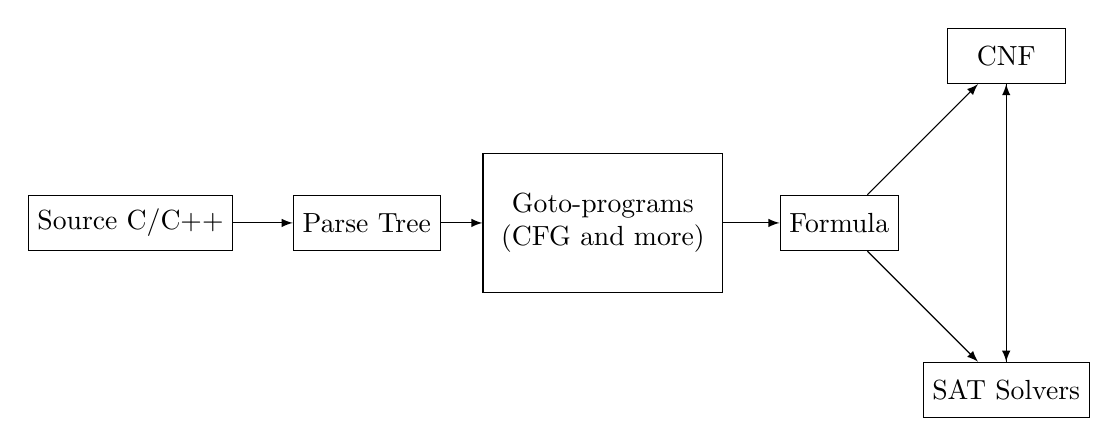
\begin{tikzpicture}[node distance=3cm, auto, >=latex]
          \node (source) [module] {Source C/C++};
          \node (parsetree) [module, right of=source] {Parse Tree};
          \node (cfg) [goto, right of=parsetree] {Goto-programs (CFG and more)};

          \node (formula) [module, right of=cfg] {Formula};
          \node (cnf) [module, above right of=formula] {CNF};
          \node (smt) [module, below right of=formula] {SAT Solvers};

          \path[line] (source) -- (parsetree);
          \path[line] (parsetree) -- (cfg);
          \path[line] (cfg) -- (formula);
          \path[line] (formula) -- (cnf);
          \path[line] (formula) -- (smt);
          \path[line] (cnf) -- (smt);
          \path[line] (smt) -- (cnf);
    \end{tikzpicture}
    \caption{Block diagram of CBMC}
    \label{fig:CBMC:block}

\end{figure}


\subsubsection{Loop Unrolling}
Loop unrolling, also called as loop unwinding, is process of converting loops into sequential statements. For example:

\begin{figure}[htbp]
    \centering
    \tikzstyle{module}=[draw, text centered, minimum height=2.5em, rounded corners]

    \begin{tikzpicture}[node distance=3cm, auto, >=latex]
    \node (source) [module] {
\begin{lstlisting}
for(i=0; i<5; i++)
{
    array_a[i] = array_b[i] + 100;
}
\end{lstlisting}
};
    \end{tikzpicture}
   \caption{An example of loop with static condition}
   \label{fig:example:loop:with:static:condition}
\end{figure}

Example \autoref{fig:example:loop:with:static:condition} can be simply converted as shown in \autoref{fig:example:unrolled:loop:with:static:condition}, which contains sequential statements.
\begin{figure}[htbp]
    \centering
    \tikzstyle{module}=[draw, text centered, minimum height=2.5em, rounded corners]

    \begin{tikzpicture}[node distance=3cm, auto, >=latex]
    \node (source) [module] {
\begin{lstlisting}
    array_a[0] = array_b[0] + 100;
    array_a[1] = array_b[1] + 100;
    array_a[2] = array_b[2] + 100;
    array_a[3] = array_b[3] + 100;
    array_a[4] = array_b[4] + 100;
\end{lstlisting}
};
    \end{tikzpicture}
   \caption{An example of unrolled loop with static condition}
   \label{fig:example:unrolled:loop:with:static:condition}
\end{figure}

Typically there are also loops which are bounded by run-time conditions, for example in \autoref{fig:example:loop:with:dynamic:condition}.
\begin{figure}[htbp]
    \centering
    \tikzstyle{module}=[draw, text centered, minimum height=2.5em, rounded corners]

    \begin{tikzpicture}[node distance=3cm, auto, >=latex]
    \node (source) [module] {
\begin{lstlisting}
while(array_b[i] != '\0')
{
    array_a[i] = array_b[i];
    i++;
}
\end{lstlisting}
};
    \end{tikzpicture}
   \caption{An example of loop with dynamic condition}
   \label{fig:example:loop:with:dynamic:condition}
\end{figure}

C code in \autoref{fig:example:loop:with:dynamic:condition} contains a while loop which terminates when array\_b encounters an end of string character ($\backslash 0$) in its index. Static analysis may not provide any information about the contents of arry\_b and it is impossible to know the number of iteration loop will run during execution. Most of the tools use bounded loop unrolling, i.e. if the exit condition for a loop cannot be determined statically, loops are unrolled a maximum of N number of times. Number N can be adjusted according to application. For instance above loop in \autoref{fig:example:loop:with:dynamic:condition}, with N set to 5, can be transformed as shown in \autoref{fig:example:unrolled:loop:with:dynamic:condition}.

\begin{figure}[htbp]
    \centering
    \tikzstyle{module}=[draw, text centered, minimum height=2.5em, rounded corners]

    \begin{tikzpicture}[node distance=3cm, auto, >=latex]
    \node (source) [module] {
\begin{lstlisting}
{
    if(array_b[i + 0] != '\0')
    {
        array_a[i + 0] = array_b[i + 0];
        if(array_b[i + 1] != '\0')
        {
            array_a[i + 1] = array_b[i + 1];
            if(array_b[i + 2] != '\0')
            {
                array_a[i + 2] = array_b[i + 2];
                if(array_b[i + 3] != '\0')
                {
                    array_a[i + 3] = array_b[i + 3];
                    if(array_b[i + 4] != '\0')
                    {
                        array_a[i + 4] = array_b[i + 4];

                        if(array_b[i + 5] != '\0')
                             assert(0);
                    }
                }
            }
        }
    }
}
\end{lstlisting}
};
    \end{tikzpicture}
   \caption{An example of unrolled loop with dynamic condition}
   \label{fig:example:unrolled:loop:with:dynamic:condition}
\end{figure}

Assert statement, at last, can be used to check if unrolling was not enough.


\subsubsection{Goto-programs}
Goto-program is compiled source code, which stores program's information in a structured way. The information includes Control Flow Graph (CFG), data types of the variable, type conversions, library functions and etc.


\subsubsection{Variable renaming}
Programs also have variables with multiple assignments on same control flow path and it adds complexity on the way we verify programs. To avoid the complexity, variables are renamed whenever new values are assigned. It is known as Static Single Assignment (SSA\index{SSA}). This process is done on goto-programs before converting programs into propositional logic. For example, source code shown in \autoref{fig:example:multiple:assignments} can be represented as: 

$ a = 10 \wedge sum = sum + a \wedge sum > MAX\_VALUE$

As we can see in the expression, $sum$ is assigned a value and used as a source in the expression. It is not possible to represent such expressions in proposition logic. To avoid it, CBMC converts logic as shown in \autoref{fig:example:renaming:varibales}.

\begin{figure}[htbp]
    \centering
    \tikzstyle{module}=[draw, text centered, minimum height=2.5em, rounded corners]

    \begin{tikzpicture}[node distance=3cm, auto, >=latex]
    \node (source) [module] {
\begin{lstlisting}
    a=10;
    ...
    sum = sum + a;
    ...
    assert(sum > MAX_VALUE)
\end{lstlisting}
};
    \end{tikzpicture}
   \caption{An example of Multiple assignments}
   \label{fig:example:multiple:assignments}
\end{figure}



\begin{figure}[htbp]
    \centering
    \tikzstyle{module}=[draw, text centered, minimum height=2.5em, rounded corners]

    \begin{tikzpicture}[node distance=3cm, auto, >=latex]
    \node (source) [module] {
\begin{lstlisting}
    a0 = 10;
    ...
    sum1 = sum0 + a0;
    ...
    assert(sum1 > MX_VALUE);
\end{lstlisting}
};
    \end{tikzpicture}
   \caption{Renaming variables}
   \label{fig:example:renaming:varibales}
\end{figure}


\subsubsection{Bit vector flattening}
After compiling a source file, we get goto-program. Next step is to verify properties of program and technique used to check these properties is called decision procedure. A decision procedure is a program which terminates with definite answer, true or false, for a decision problem. The decision procedure can decide on control flows based on previous assignments/operation. For example, decision procedure can identify if a control flow can trigger an assertion based on previous assignments and operations. 

Standard ways of implementing decision procedure is bit vector flattening followed by a call to a propositional SAT solver. In this process first step is encoding  statements from goto-program into bit vectors. Encoding variables and constants to bit vectors is a straight forward task, for example a variable X of size N, can be encoded into bit vectors b of length N. Bit vector operations have to be handled on individual bases. For example, let X, Y and Z be integer variable and a[n], b[n] and c[n] be the bit vectors for each variable respectively. For addition of two bits, we can use a one bit full adder circuit as in \autoref{fig:bitadder}. The circuit will provide us with following formula.

$S_i = (a_i + b_i + C_{in}) mod_2   \longleftrightarrow  (a_i \oplus b_i \oplus c_i)$


$C_{out} = (a_i + b_i + C_{in}) div_2   \longleftrightarrow  (a_i \cdot b_i + a_i \cdot C_{in} + b_i \cdot C_{in})$

Bit flattening is a process of transforming bit vector logic into propositional logic \cite{3540741046}. For example above bit vector logic can be converted to a propositional logic for $S_i$.

$ (a_i \vee b_i \vee \neg C_{out}) \wedge (a \vee \neg b \vee C_{in} \vee \neg C_{out}) \wedge (a \vee \neg b \vee \neg C_{in} \vee C_{out}) \wedge $

$(\neg a \vee b \vee C_{in} \vee \neg C_{out}) \wedge (\neg a \vee b \vee \neg C_{in} \vee  C_{out}) \wedge (\neg a \vee \neg b \vee C_{out})$


Similarly we can build carry chain adder for bit vectors, subtractor for subtract operation, bit wise operations etc. The multiplication, division and modulo operations generate large formulas. To handle large expressions and large operations incremental flattening is used \cite{3540741046}.

As we know from \autoref{sec:sat:solver}, a proposition logic can be verified using SAT solvers. SAT solver can work on propositional logic of program logic to verify expressions and check different properties of the program logic.



\begin{figure}
    \centering
    \tikzstyle{module}=[draw, text centered, minimum height=2.5em]
    \tikzstyle{input} = [coordinate]
    \tikzstyle{output} = [coordinate]
    \tikzstyle{line}=[draw, -latex]
    \tikzstyle{pinstyle} = [pin edge={to-,thin,black}]


    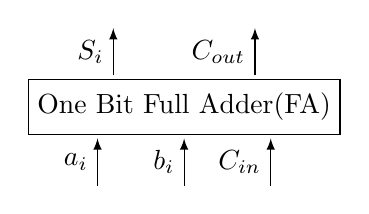
\begin{tikzpicture}[node distance=1.5cm, auto, >=latex]
          \node (input) [input] {};
          \draw [->] (-0.9, 1.9) -> node {$S_i$} (-0.9, 2.5);
          \draw [->] (0.9, 1.9) -> node {$C_{out}$} (0.9, 2.5);

          \draw [->] (-1.1, 0.5) -> node {$a_i$} (-1.1, 1.1);
          \draw [->] (0, 0.5) -> node {$b_i$} (0, 1.1);
          \draw [->] (1.1, 0.5) -> node {$C_{in}$} (1.1, 1.1);
          \node (adder) [module, above of=input] {One Bit Full Adder(FA)};
          %\draw [<-] (adder) -- node [name=b] {$b$} ;
    \end{tikzpicture}
    \caption{One Bit Full Adder (FA) \index{Full Adder}}
    \label{fig:bitadder}
\end{figure}

\begin{comment}
\begin{figure}
    \centering
    \tikzstyle{module}=[draw, text centered, minimum height=2em, minimum width = 1.5cm]
    \tikzstyle{input} = [coordinate]
    \tikzstyle{output} = [coordinate]
    \tikzstyle{line}=[draw, -latex]
    \tikzstyle{pinstyle} = [pin edge={to-,thin,black}]


    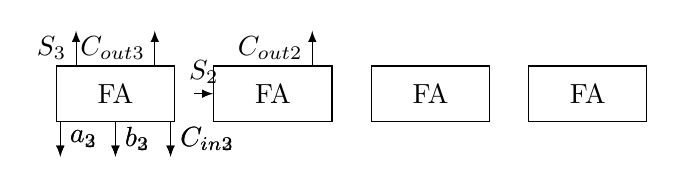
\begin{tikzpicture}[node distance=2cm, auto, >=latex]
          \node (adder1) [module] {FA};
          \node (adder2) [module, right of=adder1] {FA};
          \node (adder3) [module, right of=adder2] {FA};
          \node (adder4) [module, right of=adder3] {FA};

          \draw [->] (-0.5, 0.35) -> node {$S_3$} (-0.5, 0.8);
          \draw [->] (0.5, 0.35) -> node {$C_{out3}$} (0.5, 0.8);

          \draw [->] (-0.7, -0.35) -> node {$a_3$} (-0.7, -0.8);
          \draw [->] (0, -0.35) -> node {$b_3$} (0, -0.8);
          \draw [->] (0.7, -0.35) -> node {$C_{in3}$} (0.7, -0.8);

          \draw [->] (adder2){}+(-1,-0) -> node {$S_2$} (adder2);
          \draw [->] (2.5, 0.35) -> node {$C_{out2}$} (2.5, 0.8);

          \draw [->] (-0.7, -0.35) -> node {$a_2$} (-0.7, -0.8);
          \draw [->] (0, -0.35) -> node {$b_2$} (0, -0.8);
          \draw [->] (0.7, -0.35) -> node {$C_{in2}$} (0.7, -0.8);

          %\draw [<-] (adder) -- node [name=b] {$b$} ;
    \end{tikzpicture}
    \caption{Carry chain adder}
    \label{fig:eightadder}

\end{figure}
\end{comment}


\subsubsection{CBMC keywords}
Apart from automatically checking properties of program, CBMC also provides set of keywords, which can be used to aide CBMC with more information about program. These keywords can be used for programs instrumentation. The program instrumentation is a procedure change or adds part code to verify some properties of the code.

\begin{enumerate}
\item $assert(expr)$ or $\_\_CPROVER\_assert(expr)$ can be used to assert on any condition. It takes a Boolean expression $expr$ as argument. When CBMC encounters one of these keywords, it tries to generate a formula to check assertion failure. Generated formula is verified using SAT-solvers. If the formula is satisfied then assertion fails and CBMC generates error and produces counter-example showing possible trace of error.
\item $\_\_CPROVER\_assume(expr)$  keyword reduces the number of program traces that are considered and allows assume-guarantee reasoning. As $assert$, $\_\_CPROVER\_assume(expr)$ also takes a Boolean expression \cite{clarke2006ansi}.
\end{enumerate}

\subsubsection{Use cases of CBMC}
CBMC was used in several case studies, including Bounded Model Checking of Concurrent Programs \cite{Rabinovitz05boundedmodel}, Equivalence Checking \cite{Staats:2008:PTV:1482985.1483006}, Worst Case Execution Time analysis \cite{springerlink:10.1007/978-3-540-88479-8_30, Kim_usinga} and many other can be found in \cite{website:cprover:cbmc:applications}.


\section{Verifying properties of thread local and concurrent threads}

Model checking is also used to verify specific properties of a system. Some properties are local to a single thread running in the system and some depend on multiple threads running concurrently. The software concurrency in a single core system is introduced by context switches and parallel computing platforms have concurrent execution paths.

Thread local properties include memory access mechanisms, correctness of memory management and pattern of mutex accesses. For example work done in \cite{Donaldson:2011:AAD:2034876.2034900} is used to identify DMA race conditions in IBM cell processors. In this case study, DMA race detection is achieved through \emph{program instrumentation}. In program instrumentation, a part of code is added or modified to verify some properties of the logic. For example, to verify array bound, one can add an assertion to check the index value on every array access.

In concurrent programs we can observe more complex properties. For example, concurrent access to shared resources, signalling between the threads and dynamic memory management among threads or race conditions among the threads. Behaviour of these properties depends on the hardware and operating system support. The program instrumentation can be used to verify these properties.



\chapter{Related work}\label{sec:verification:tech}

Initially logical systems were verified using proof based systems. In proof based verification, system description is represented using a set of formulas $\gamma$ in a suitable logic and specification is represented using another formula $\theta$. The verification of system is done by finding proof that $\gamma$ $\vdash$ $\theta$. As we can see this process is deductive and usually requires human guidance \cite{Hoare04communicatingsequential, Apt:1981:TYH:357146.357150}.

%Later in 1981 model checking techniques as shown in \cite{Clarke86automaticverification}, proved that model checking can lead to algorithmic and automatic verification process. Model checking is also much simpler since it models a hardware or software description into constrained model with finite states and verifies the models instead of implementation, which hides the complexities of descriptive languages.

The work done by Vardi and Wolper in \cite{VardiW86}, provided a way of modelling the program specifications into formulas which can be verified automatically. According to this proposal, once expected behaviours and use cases are decided, all the requirements are written into formal specification, which is mathematical description of the system. The formal specifications are written in Linear time Temporal Logic (LTL) and the LTL logic are verified to check the properties of the system. If the system described using LTL behaves as expected, the system is said to be bug free.

Currently we have techniques to convert programs described in high level programming language to mathematical formulas and automated verification technique to verify the properties of the formulas. The \autoref{sec:back:cbmc} describes more details of converting programs to verifiable mathematical formulas and verification using Bounded Model Checking.

Specifications and program are converted into mathematical formulas and the formulas have to be verified for correctness and/or check for incorrect behaviour. For example consider model checking of state-machine in \autoref{fig:example:statemachine}. State $S_3$ can be reached through $S_1$ and $S_2$ under the condition $(\neg X \vee Z) \wedge (Z \wedge Y)$. Suppose we want to know if $S_3$ is reachable under certain conditions, which may violate the specification and is an incorrect behaviour. We need techniques to process the formula $(\neg X \vee Z) \wedge (Z \wedge Y)$ and check if it is satisfiable. Such techniques are called \emph{decision procedures}. Two of the commonly used decision procedures are \emph{Binary Decision Diagrams (BDDs)} and \emph{Satisfiability (SAT)} \cite{kroening2008decision}. In previous chapter we have discussed about satisfiability and next section describes BDD briefly.

``A program verifier uses automated mathematical and logical reasoning to check the consistency of programs with their internal and external specifications" \cite{Hoare03theverifying}. Hardware and software verification considers checking the correctness of functionality and finding undesired behaviours in the designed logic. There are several stages and ways in which a system can be verified. During the design process a system specification is developed and a mathematical model can be implemented to verify if the properties of specified system are as expected. The implemented logic can be converted into mathematical logic and this mathematics logic can be verified for its correctness. There are already tools which can work with system specifications like UML and automatons. For example \href{http://move.lip6.fr/software/BCC/index.html}{BCC} and \href{http://www.uppaal.com/}{UPPAAL}. Also there are tools which can work with implementation done in programming languages like C, C++, Verilog or VHDL. For example, \href{http://www.cprover.org/cbmc/}{CBMC}, \href{http://www.cprover.org/satabs/}{SatAbs} and \href{http://www.cs.cmu.edu/~modelcheck/vcegar/}{VCEGAR}. 
\subsection{Binary Decision Diagrams (BDDs)}

\index{BDD}\index{DAG}Graph based verification techniques like \emph{Binary Decision Diagrams (BDDs)}, as described in \cite{Bryant:1986:GAB:6432.6433}. The BDDs are proven to be very effective in verifying binary logic \cite{brace1991efficient}. In this approach the model is described in-terms of a Directed Acyclic Graph (DAG) consisting of decision nodes and terminal nodes. 


\begin{comment}
The terminal nodes can be either 0 or 1 and the decision nodes, with out-degree 2, are nodes combining the terminal 0's or 1's or a combination decision nodes. The left edge going out from the decision node represents case when a variable is 0 and right edge represents the case for 1. 

\autoref{fig:example:bdd} shows a BDD for state machine in \autoref{fig:example:statemachine}, containing decision nodes $X$, $Y$ and $Z$. The terminal nodes containing 0 or 1 based on the evaluation of the formula $(\neg X \vee Z) \wedge (Z \wedge Y)$. The reach-ability analysis on BDD-DAG provides facilities to check if a particular behaviours is possible in the system. For example we can check if $S_3$ is reachable if $Z$ is 0 and it is not possible since all the left edges from Z reach a 0 terminal node. There are various tools like \href{http://fmv.jku.at/abcd/}{ABCD}, \href{http://move.lip6.fr/software/BCC/index.html}{BCC} and \href{http://www.jossowski.de/projects/jinc/jinc.html}{JINC} which can be used to verify programs using BDD.

\begin{figure}[htbp]
   \centering
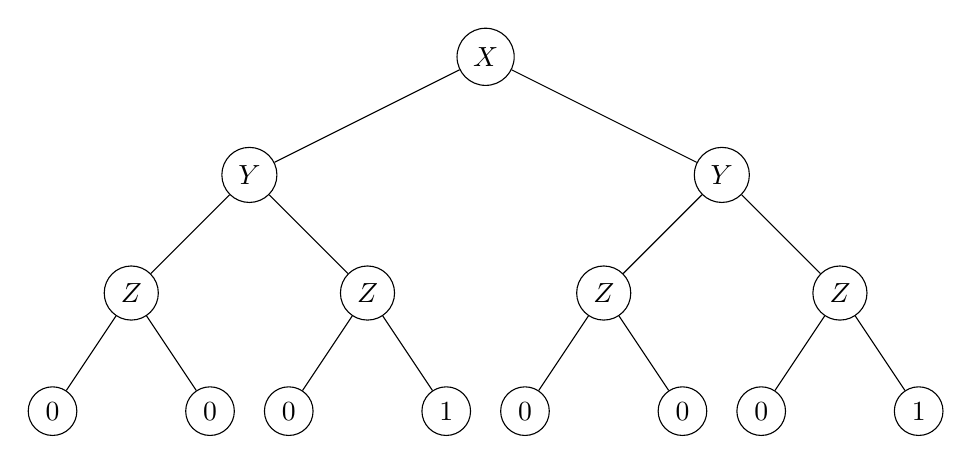
\begin{tikzpicture}[level/.style={sibling distance=60mm/#1}]
\node (z)[circle,draw] {$X$}
      child {node [circle,draw] (ab) {$Y$}
        child {node [circle,draw] (a) {$Z$}
          child {node [circle,draw] {$0$}}
          child {node [circle,draw] {$0$}}}
        child {node [circle,draw] (b) {$Z$}
          child {node [circle,draw] {$0$}}
          child {node [circle,draw] {$1$}}}}
      child {node [circle,draw] (cd) {$Y$}
        child {node [circle,draw] (c) {$Z$}
          child {node [circle,draw] {$0$}}
          child {node [circle,draw] {$0$}}}
        child {node [circle,draw] (d) {$Z$}
          child {node [circle,draw] {$0$}}
          child {node [circle,draw] {$1$}}}};

   \end{tikzpicture}
   \caption{Binary Decision Diagram (BDD)}
   \label{fig:example:bdd}
\end{figure}

\end{comment}

Although BDDs are effective in solving verification problem, as the number of variables/nodes increase the size of BDDs increases exponentially and it is not practical to use BDDs, since verification process will be too slow and too memory consuming \cite{clarke1997model}. There have been attempts to develop techniques which can avoid the exponential growth, for instance work shown in \cite{Burch90symbolicmodel, Balarin:1993:IAL:647762.735495, Pixley:1992:ECS:113938.149645} and work by Bryant in \cite{Bryant:1986:GAB:6432.6433} showed that ordering variables will increase the efficiency of the algorithm. But despite all the efforts state explosion has been a major hurdle in applying BDD-based model checking to large and complex systems \cite{springerlink:10.1007-3-540-44577-3-12}.

